\chapter{Discussion} \label{sec:DISCUSSION}

We tested the implementation with two JavaScript benchmark suites and our target programming system, the Lively Kernel.
The proxies, which implement version-aware references, behave like the respective versions of objects in all situations exhibited.
The linear global runtime versions allows to re-establish previous development states in Lively.
That is, all references to relevant objects appear to be version-aware references in the tested situations.

The memory overhead of our implementation appears to be practical, while the execution overhead of the current implementation does not.
The measured execution overhead is in the range of three orders of magnitude for popular JavaScript benchmarks and typical user interactions in Lively.
Direct comparisons of just the version-aware references and direct references show slow downs of four orders of magnitude.
In analyzing these results, we gained the impression that only one order of magnitude is due to the specific proxy behavior, while most of the overhead can be ascribed to the Direct Proxies as currently available in the Chrome browser.
In fact, a comparable indirection can be implemented considerably faster with ordinary JavaScript and further source transformations, promising more practical implementations.

\todo{Eval: should we add something about how long it takes to do the source transformations?}
\todo{Eval: should we add something on how long commit and undo/redo take?}

\section{Functionality: Undo and Redo for the Lively Kernel}

Besides testing the behavior of our proxies and our source transformations with isolated test cases, we also used two benchmark suites to check our implementation.
In particular, the system works for all benchmarks from the Octance benchmark suite\footnote{\url{http://code.google.com/p/octane-benchmark/},\goodbreak accessed February 3, 2014, at version 26} and the JavaScript version of the Computer Language Benchmarks Game\footnote{\url{http://benchmarksgame.alioth.debian.org/},\goodbreak accessed February 3, 2014}, javascript implementation\footnote{\url{http://github.com/kragen/shootout},\goodbreak accessed February 3, 2014, at version 71aa4ec4cd15940c59f1a1bb71ac1ff1572a55c2}.
For each individual benchmark, we transform the source code using our source transformations and, thereby, execute the benchmark code with version-aware references to mutable objects.
All benchmarks run without errors and return the same results as when executed without any source transformations.
These tests indicate that the source transformation yields working source code and that our proxy-based version-aware references behave as intended where used.
For the questions whether all references to mutable objects are version-aware and whether the version-aware references correctly delegate to one among many versions---that is, whether the source transformations and proxies allow to preserve and re-establish versions of Lively's JavaScript runtime---we tested the simple linear runtime versioning explained in \todo{3.2.3..}:
When we pass Lively's source code modules to our source transformations during the bootstrap, we were able to preserve and re-establish the particular runtime state of multiple example scenarios, including the state of graphical applications of, for example, text editors and other developer tools.
That is, at least for the scenarios we tested, our approach and its proxy-based JavaScript implementation provides fine-grained object versioning for the Lively Kernel.

\todo{only the v8 benchmark suite, as language shootout actually contains too many benchmarks...!!}
\todo{add some info about the reduced input sizes to the Splay benchmark.. input reduced by one order of magnitude.. as automatic execution was impeded by unresponsive JS script check otherwise.. }

\todo{should we add a link to a published demo screencast for this? or screenshots? and describe the tested undo/redo scenarios a bit more..?}


\section{Practicability: Impact on Performance}

memory overhead: for the version-aware references, but the overhead does increase with the number of versions per object...
\begin{itemize}
    \item for the version-aware references for lively, measured (and explained… per proxy now...)
    \item something about how each new global version requires memory, but each depending on how big the changes are / or how much needs to be copied..
\end{itemize}

\todo{should we also present some numbers for how much more memory is consumed when we create versions?}

\begin{figure}[h]
    \centering
    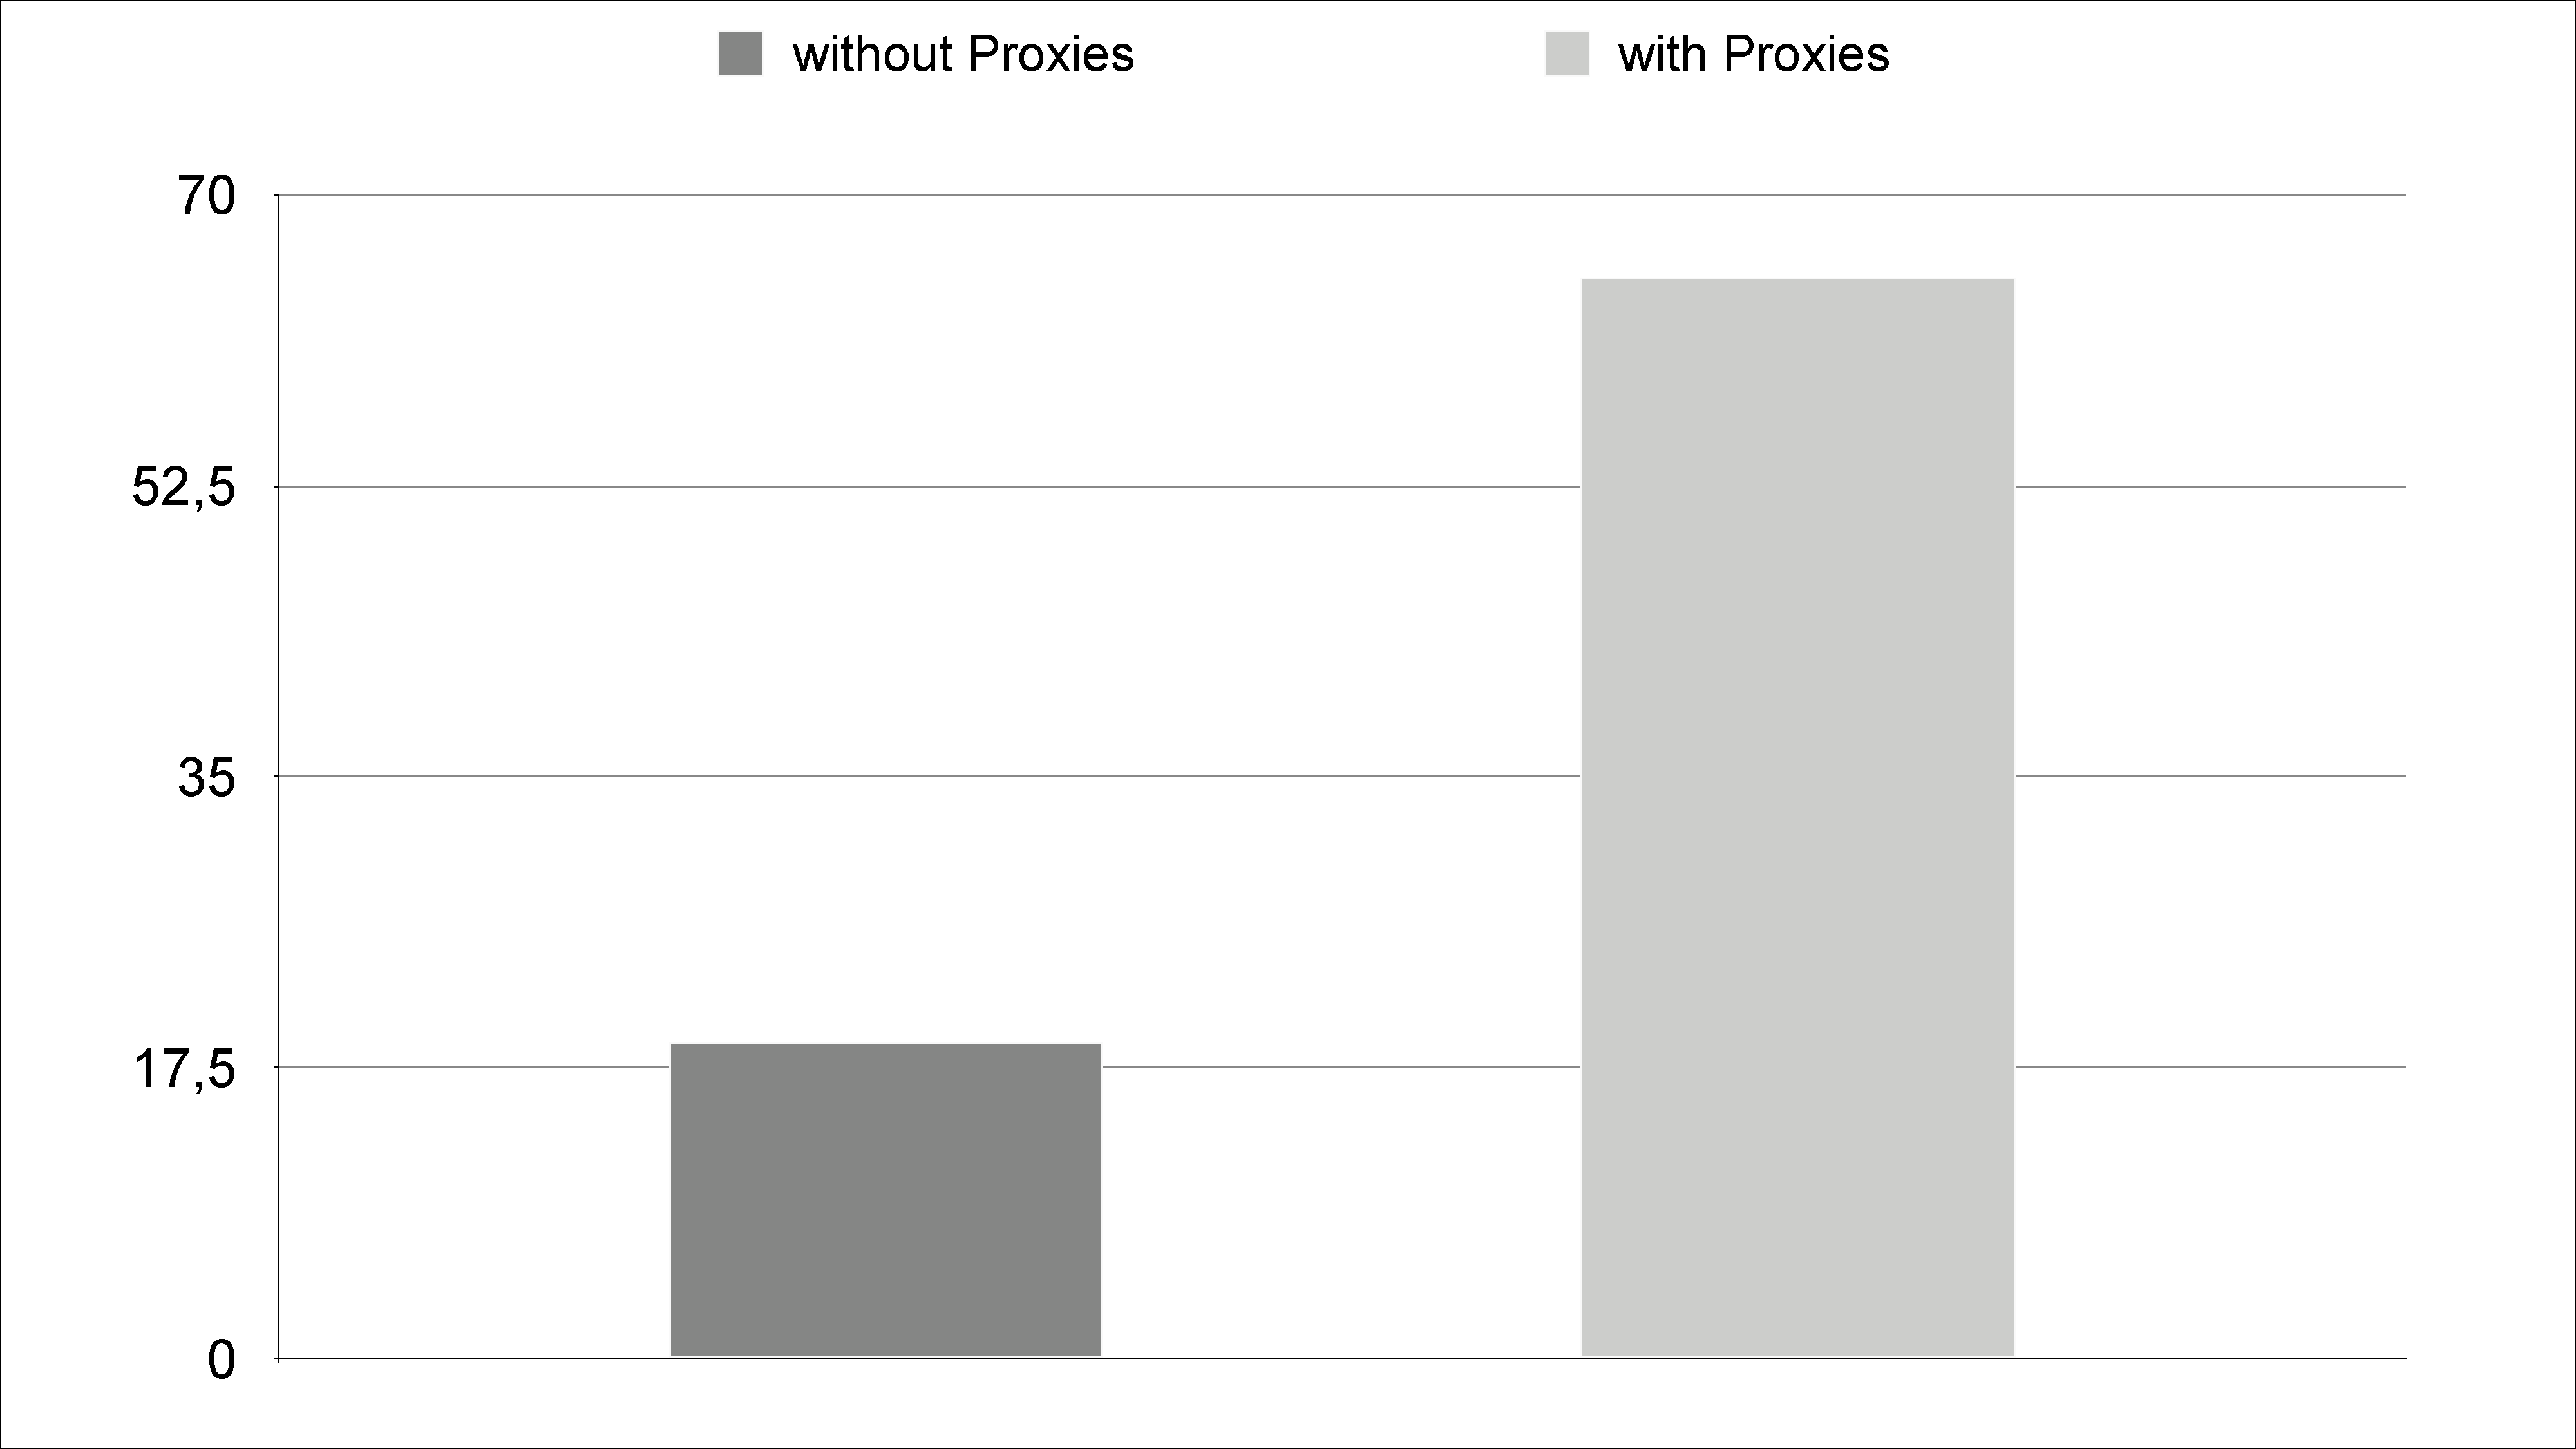
\includegraphics[width=\textwidth]{figures/memoryOverhead.pdf}
    \caption{Memory consumption when starting an empty Lively Kernel environment in megabyte.}
    \label{fig:ExecutionOverhead}
\end{figure}

execution time overhead: for the version-aware references, and the overhead does not increase with the number of versions per object...
\begin{itemize}
    \item common JavaScript language benchmark suites – with vs. without proxies.. see Figure~\ref{fig:ExecutionOverheads}
    \item user interaction benchmarks – with vs. without proxies: starting the lively kernel (including loading a world), opening halos on a morph, opening the world menu, opening the parts bin (/ a workspace / the system code browser), resizing the SCB (programmatically) (?), dragging (programmatically) (?)
\end{itemize}


\begin{figure}[h]
    \centering
    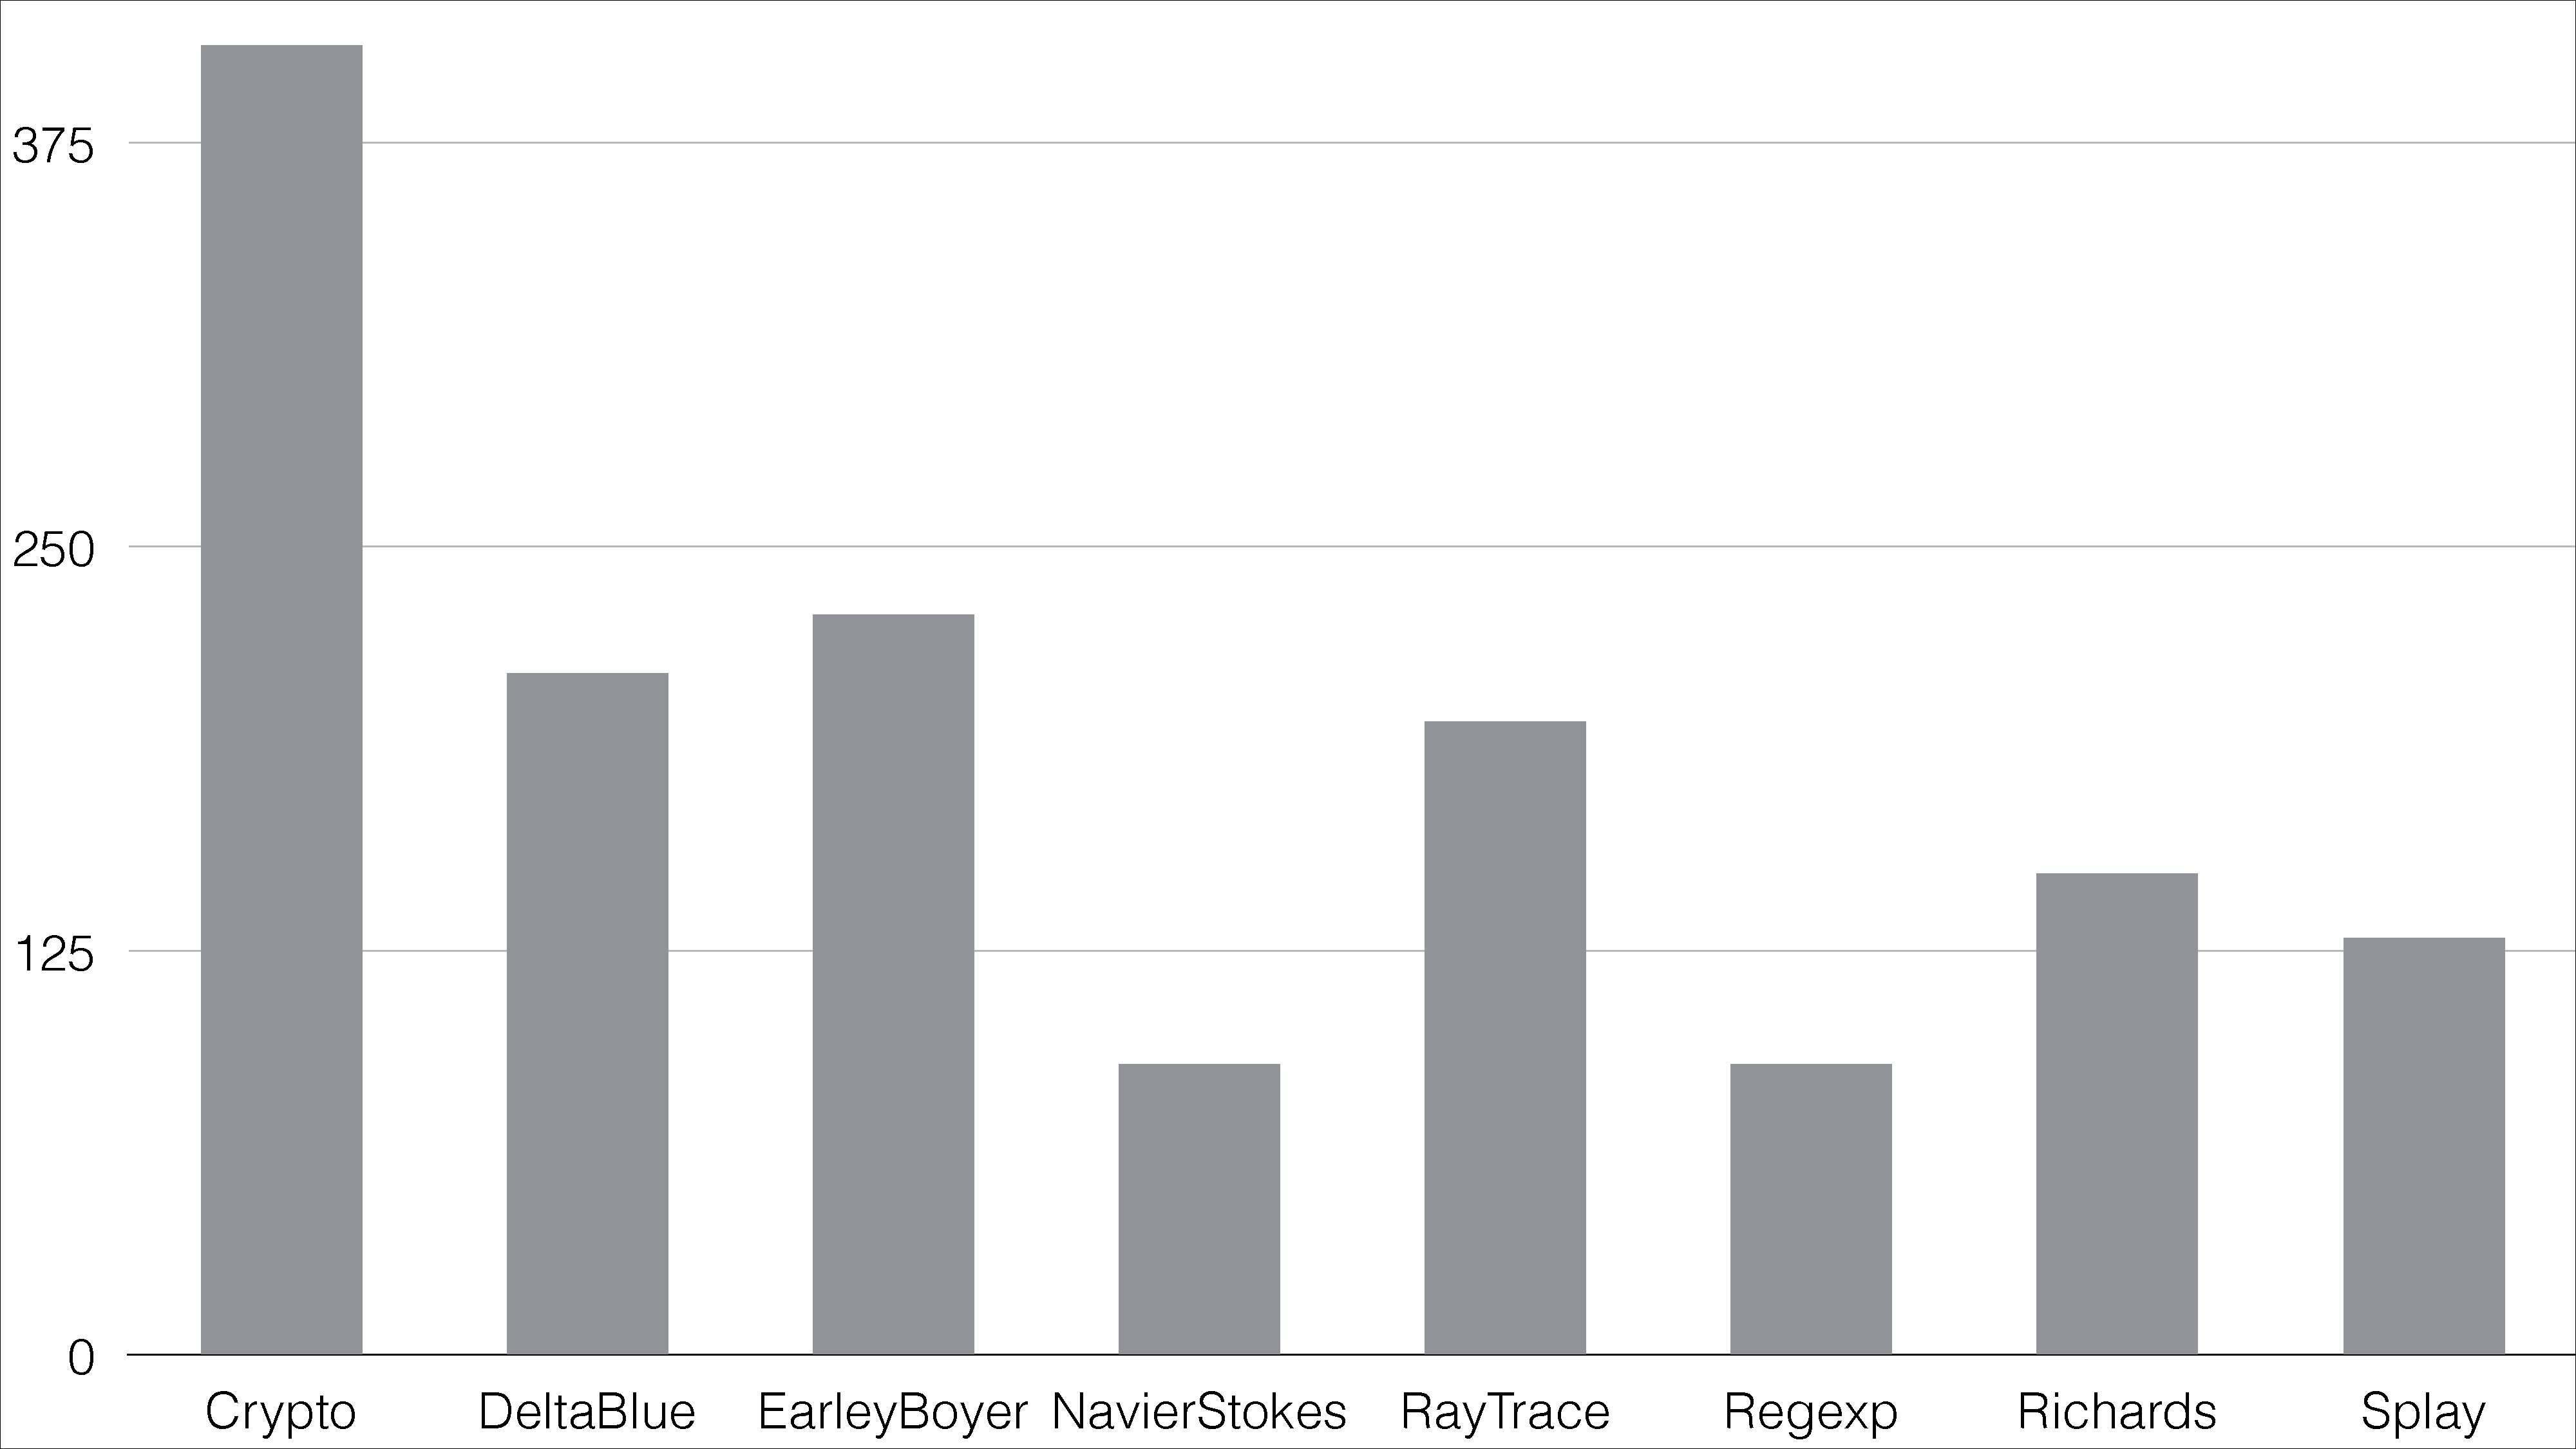
\includegraphics[width=\textwidth]{figures/executionOverhead.pdf}
    \caption{Execution overhead for proxy-based version-aware references in 100\% overhead compared to ordinary JavaScript references.}
    \label{fig:ExecutionOverhead}
\end{figure}



analysis...
maybe some discussion of the execution overhead and numbers on the different layers of the layered implementation cost how much performance: versioning proxy handler > default ES 6 shim proxies > harmony proxies in Chrome..

% This raises questions about the current state of the implementation of the proxies themselves, especially about interference with the v8's JIT compiler, and also indicates more practical implementation strategies.


% say something about how much time it takes to commit and re-establish a version?